\documentclass[conference]{IEEEtran}
\IEEEoverridecommandlockouts
% The preceding line is only needed to identify funding in the first footnote. If that is unneeded, please comment it out.
%Template version as of 6/27/2024

\usepackage{cite}
\usepackage{amsmath,amssymb,amsfonts}
\usepackage{algorithmic}
\usepackage{graphicx}
\usepackage{textcomp}
\usepackage{xcolor}
\def\BibTeX{{\rm B\kern-.05em{\sc i\kern-.025em b}\kern-.08em
    T\kern-.1667em\lower.7ex\hbox{E}\kern-.125emX}}
\begin{document}

\title{Algorithm Selection and Auto-Tuning in AutoPas}

\author{
    \IEEEauthorblockN{ Manuel Lerchner}
    \IEEEauthorblockA{
        \textit{Technical University of Munich}\\
        Munich, Germany}
}

\maketitle

\begin{abstract}
    TODO
\end{abstract}

\begin{IEEEkeywords}
    TODO, TODO, TODO
\end{IEEEkeywords}


\section{Introduction}
Todo introduction \cite{test}.

\begin{figure}[htbp]
    \centerline{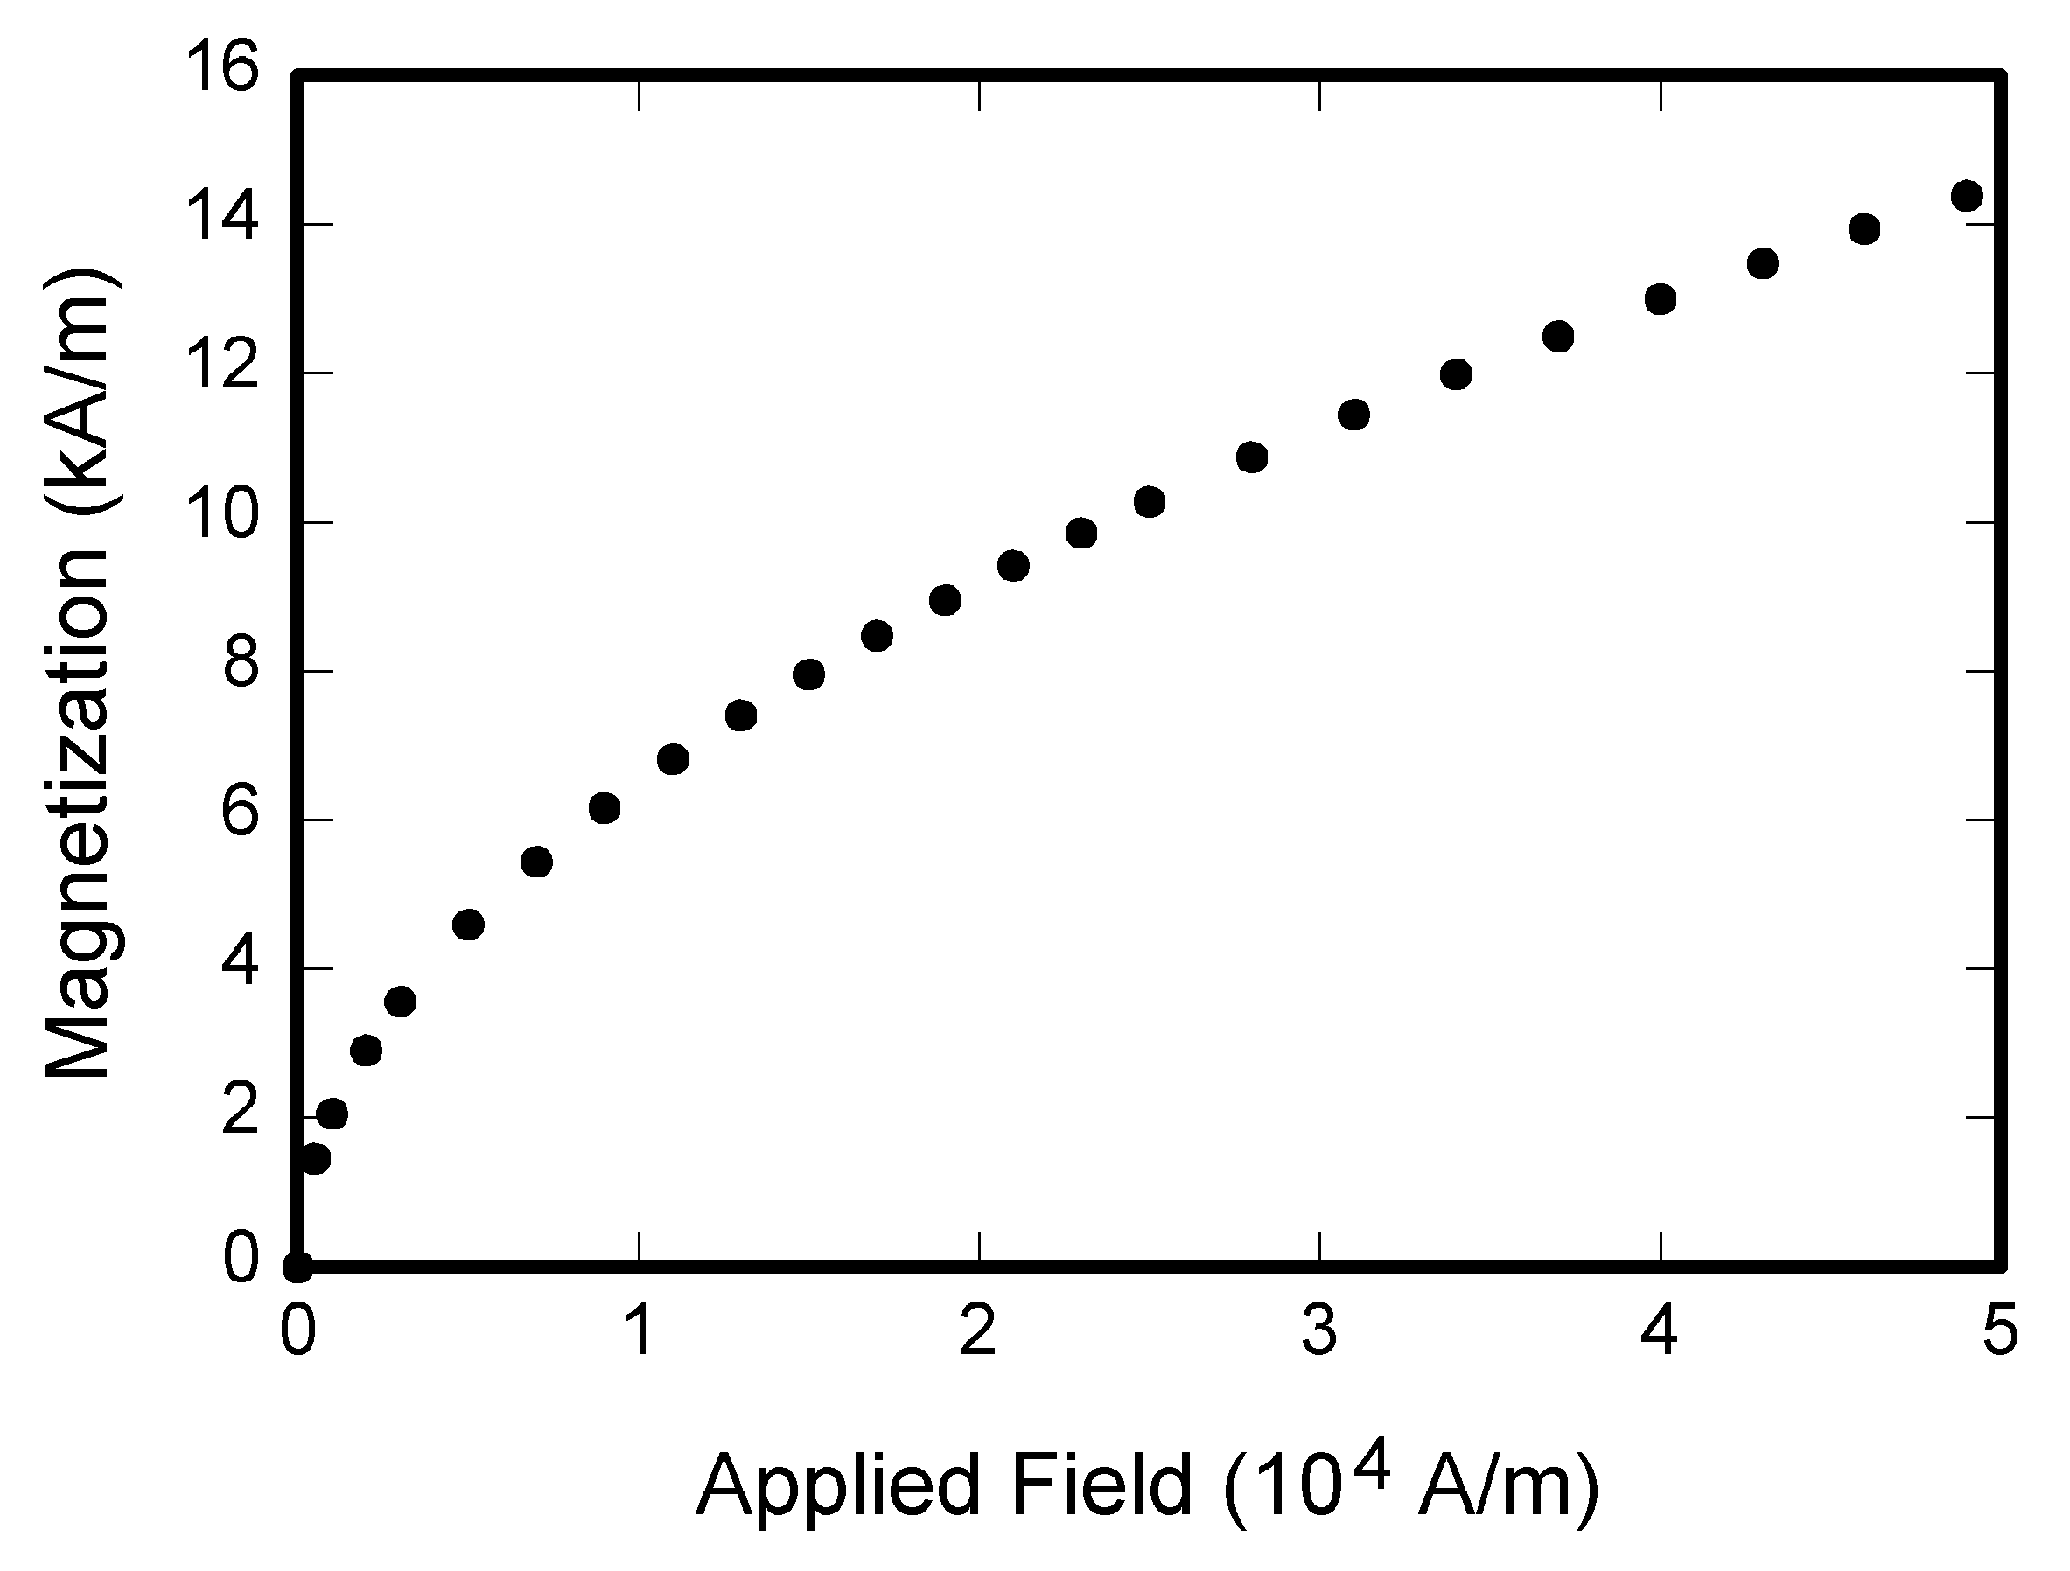
\includegraphics{figures/fig1.png}}
    \caption{Example of a figure caption.}
    \label{fig}
\end{figure}


\section*{References}

\bibliographystyle{plain}
\bibliography{refs}

\end{document}
